\documentclass[12pt,a4paper]{article}
\usepackage[utf8]{inputenc}
\usepackage{amsmath, amssymb, physics}
\usepackage{geometry}
\usepackage{hyperref}
\usepackage{tikz}
\usepackage{setspace}
\geometry{margin=2cm}
\setstretch{1.2}

\title{O Coração da Mecânica Quântica e sua Extensão à QFT}
\author{Samuel Keullen Sales}
\date{\today}

\begin{document}

\maketitle

\section*{1. Introdução}
A equação de Schrödinger descreve a evolução temporal de estados quânticos. Para uma partícula unidimensional:

\begin{equation}
i \hbar \frac{\partial}{\partial t} \Psi(x,t) = \hat{H} \Psi(x,t)
\end{equation}

\begin{itemize}
    \item \(\Psi(x,t)\): função de onda da partícula.
    \item \(\hat{H}\): Hamiltoniano do sistema.
    \item \(|\Psi(x,t)|^2\): densidade de probabilidade de encontrar a partícula na posição \(x\) no instante \(t\).
\end{itemize}

\section*{2. Equação de Schrödinger aplicada a uma função de onda}
Exemplo: poço infinito 1D
\[
\hat{H} = -\frac{\hbar^2}{2m} \frac{\partial^2}{\partial x^2}, \quad 0 < x < L
\]

Soluções estacionárias:
\[
\psi_n(x) = \sqrt{\frac{2}{L}} \sin\frac{n \pi x}{L}, \quad E_n = \frac{n^2 \pi^2 \hbar^2}{2 m L^2}, \quad n=1,2,3,\dots
\]

\section*{3. Mecânica Quântica de Campos (QFT)}
Na QFT, a função de onda \(\Psi(x,t)\) é substituída por um operador de campo \(\hat{\phi}(x,t)\):

\begin{equation}
\hat{H} = \int d^3x \, \left[ \frac{1}{2} \hat{\pi}^2(x) + \frac{1}{2} (\nabla \hat{\phi}(x))^2 + \frac{1}{2} m^2 \hat{\phi}^2(x) \right]
\end{equation}

\begin{itemize}
    \item \(\hat{\phi}(x)\): operador de campo no ponto \(x\).
    \item \(\hat{\pi}(x) = \frac{\partial \hat{\phi}}{\partial t}\): momento conjugado do campo.
    \item Cada modo do campo equivale a um oscilador harmônico quântico.
\end{itemize}

Estado geral do sistema:
\begin{equation}
\ket{\Psi} = \sum_{n_0,n_1,\dots} c_{n_0,n_1,\dots} \ket{n_0, n_1, \dots}
\end{equation}

\section*{4. Analogias e Aplicação}

\begin{itemize}
    \item Uma partícula: função de onda \(\Psi(x,t)\).
    \item Um campo: conjunto de funções de onda \(\hat{\phi}(x,t)\), cada modo com sua própria energia e número de partículas.
    \item Probabilidade de detectar partículas em posições específicas obtida por operadores densidade: \(\hat{n}(x) = \hat{\phi}^\dagger(x)\hat{\phi}(x)\).
\end{itemize}

\begin{figure}[h!]
\centering
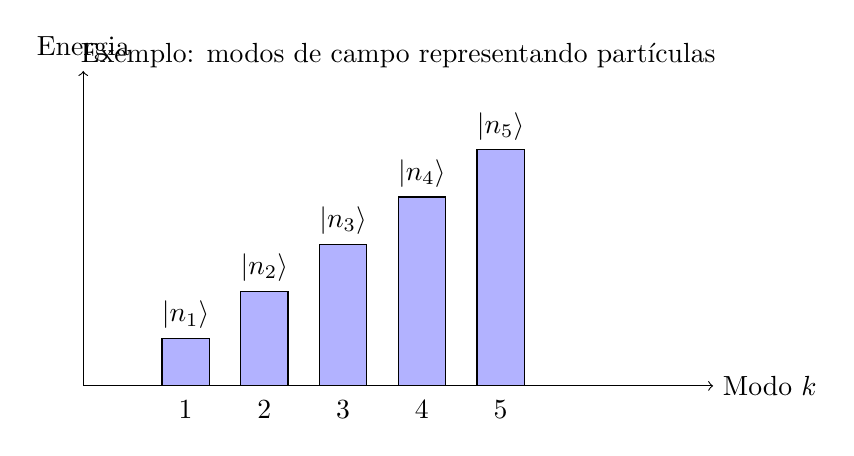
\begin{tikzpicture}[scale=1]
    % Eixos
    \draw[->] (0,0) -- (8,0) node[right]{Modo \(k\)};
    \draw[->] (0,0) -- (0,4) node[above]{Energia};
    
    % Modos do campo
    \foreach \x in {1,2,3,4,5} {
        \draw[fill=blue!30] (\x,0) rectangle (\x+0.6,\x*0.6);
        \node at (\x+0.3, -0.3) {\(\x\)};
        \node at (\x+0.3, \x*0.6 + 0.3) {\(\ket{n_\x}\)};
    }
    
    \node at (4,4.2) {Exemplo: modos de campo representando partículas};
\end{tikzpicture}
\caption{Cada modo do campo é equivalente a um oscilador harmônico quântico.}
\end{figure}

\section*{5. Experimento Mental do Gato em QFT}

Superposição de estados:
\[
\ket{\Psi_\text{gato}} = \alpha \ket{\text{vivo}} + \beta \ket{\text{morto}}
\]

Na QFT:
\[
\ket{\Psi_\text{campo}} = c_0 \ket{0_\text{fótons}} + c_1 \ket{1_\text{fóton}} + \dots
\]

\begin{itemize}
    \item Cada estado do campo equivale a diferentes configurações possíveis do experimento.
    \item Evolução temporal segue:
    \[
    i \hbar \frac{\partial}{\partial t} \ket{\Psi_\text{campo}} = \hat{H}_\text{campo} \ket{\Psi_\text{campo}}
    \]
    \item Possibilita ``pensar'' o experimento matematicamente.
\end{itemize}

\section*{6. Conclusão}

\begin{itemize}
    \item A equação de Schrödinger é a base da MQ.
    \item Em QFT, cada partícula é substituída por modos de campo, mantendo a natureza probabilística da MQ.
    \item Superposição de estados é natural e pode ser formalizada matematicamente.
    \item Figuras e equações ajudam a visualizar o campo como conjunto de osciladores quânticos.
\end{itemize}

\end{document}
